% ------------------------------------------------------------------------------
% TYPO3 CMS 8.0 - What's New (English Version)
%
% @author	Patrick Lobacher <patrick@lobacher.de> and Michael Schams <schams.net>
% @license	Creative Commons BY-NC-SA 3.0
% @link		http://typo3.org/download/release-notes/whats-new/
% @language	English
% ------------------------------------------------------------------------------
% LTXE-CHAPTER-UID:		d71b4b88-f79b2343-d2b356bf-452cef81
% LTXE-CHAPTER-NAME:	Backend User Interface
% ------------------------------------------------------------------------------

\section{Backend User Interface}
\begin{frame}[fragile]
	\frametitle{Backend User Interface}

	\begin{center}\huge{Kapitel 1:}\end{center}
	\begin{center}\huge{\color{typo3darkgrey}\textbf{Backend User Interface}}\end{center}

\end{frame}

% ------------------------------------------------------------------------------
% LTXE-SLIDE-START
% LTXE-SLIDE-UID:		d8599a04-11b4fa8c-9be5812a-715820e1
% LTXE-SLIDE-ORIGIN:	ef1d6d8c-0db67396-dedb5814-1767169f German
% LTXE-SLIDE-TITLE:		Recover pages recursively to top of rootline
% LTXE-SLIDE-REFERENCE:	!Feature-1835-RecoverPagesRecursivelyToTop.rst
% ------------------------------------------------------------------------------
\begin{frame}[fragile]
	\frametitle{Backend User Interface}
	\framesubtitle{Rekursive Wiederherstellung von Seiten}

	Das Modul "Recycler" unterstützt nun die rekursive Wiederherstellung von gelöschten Seiten zurück bis zum ersten Level der Rootline.

	Dieses Feature ist auschließlich für Admin-User verfügbar, da hierfür spezielle Rechte vorhanden sein müssen.

	\begin{figure}
		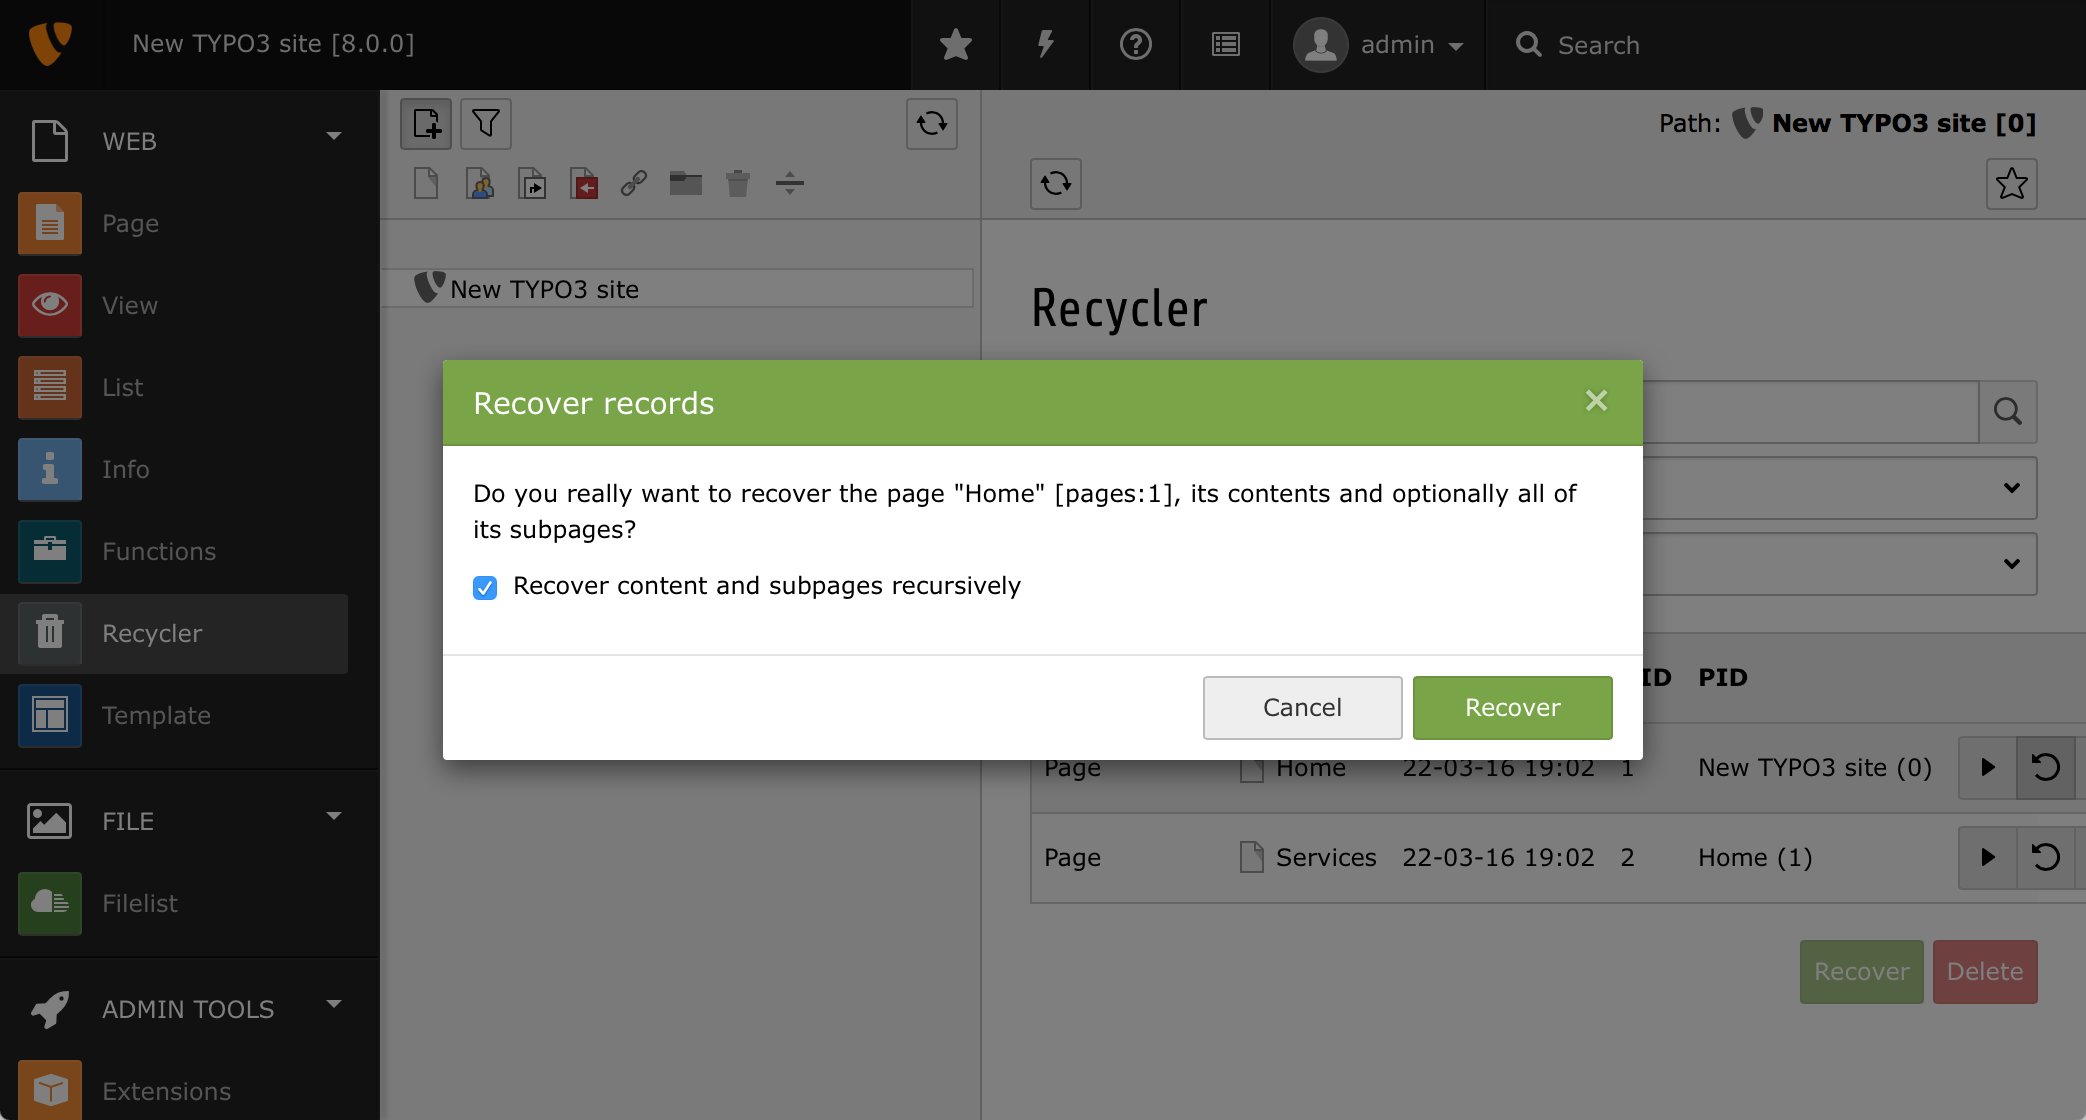
\includegraphics[width=0.70\linewidth]{BackendUserInterface/1835.png}
	\end{figure}

\end{frame}

% ------------------------------------------------------------------------------
% LTXE-SLIDE-START
% LTXE-SLIDE-UID:		04855567-dac16e24-f5274c64-f1d49c36
% LTXE-SLIDE-TITLE:		EXT:form - Directly load form wizard as inline wizard
% LTXE-SLIDE-REFERENCE:	!Feature-69394-EXTform-DirectlyLoadFormWizardAsInlineWizard.rst
% ------------------------------------------------------------------------------
\begin{frame}[fragile]
	\frametitle{Backend User Interface}
	\framesubtitle{Form-Assistent als Inline-Wizard}

	Der Assistent der Extension \texttt{EXT:form} wird nun direkt inline geladen.
	Früher musste man hierzu das Content-Element speichern und Neuladen, um den Assistenten zu verwenden.

	\begin{figure}
		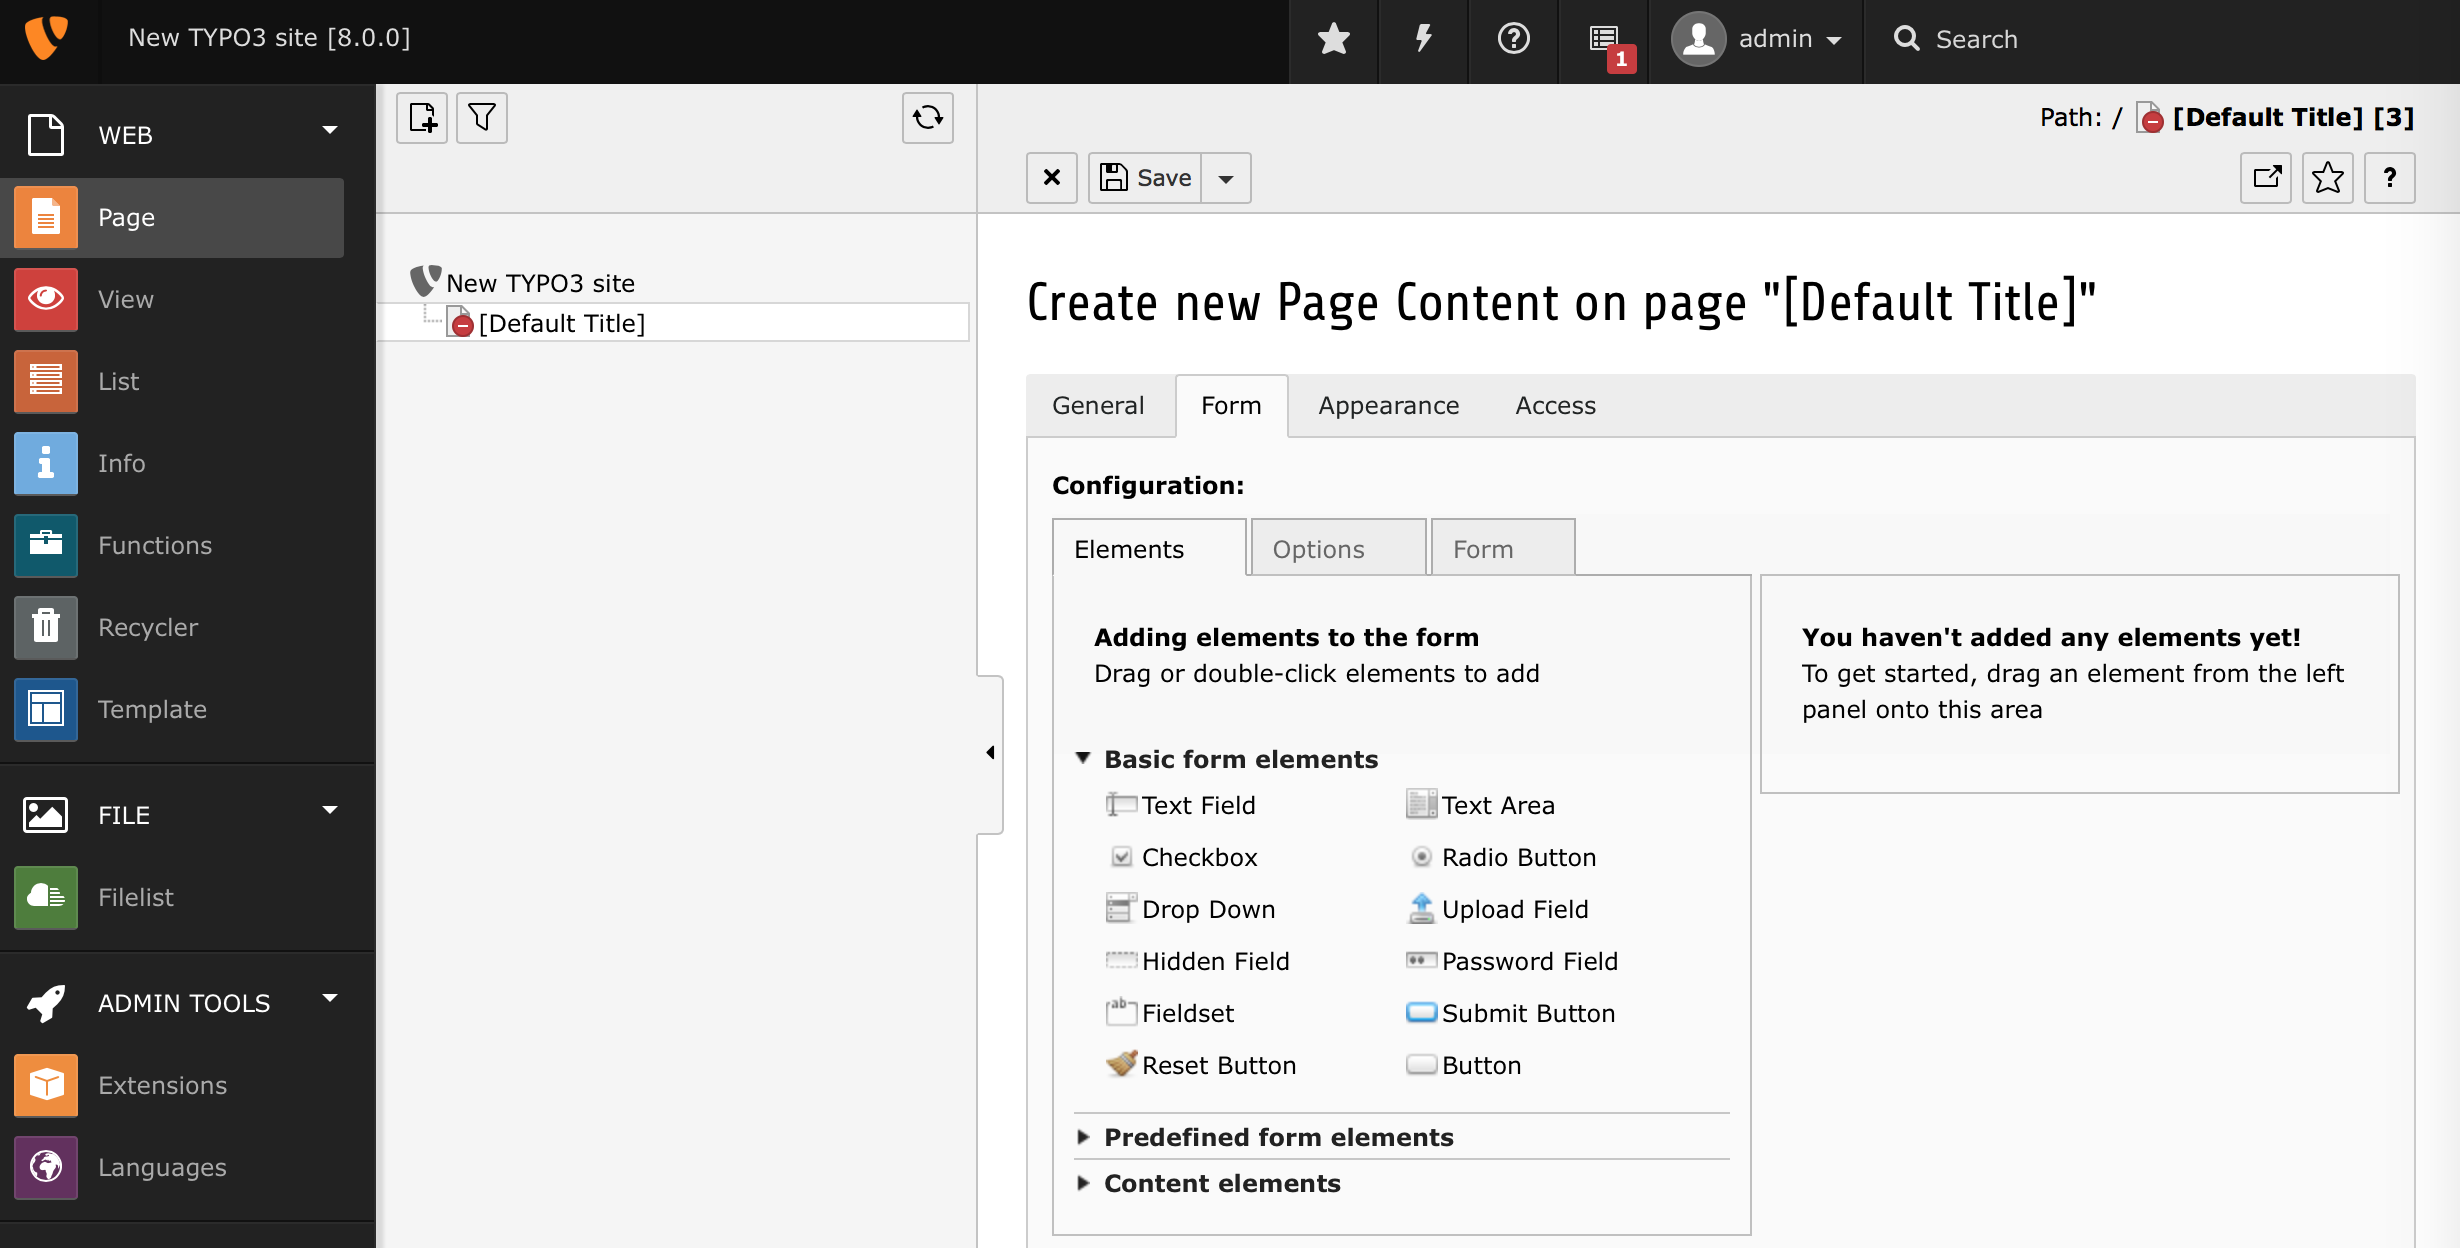
\includegraphics[width=0.70\linewidth]{BackendUserInterface/69394.png}
	\end{figure}

\end{frame}

% ------------------------------------------------------------------------------
% LTXE-SLIDE-START
% LTXE-SLIDE-UID:		fd6d762a-b268caf0-cb6f9195-f553e035
% LTXE-SLIDE-TITLE:		Set the alternative backend logo via Extension Manager
% LTXE-SLIDE-REFERENCE:	!Feature-74109-SetTheAlternativeBackendLogoViaExtensionManager.rst
% ------------------------------------------------------------------------------
\begin{frame}[fragile]
	\frametitle{Backend User Interface}
	\framesubtitle{Setzen eines alternativen Backend-Logos via Extension Manager}

	Das Backend-Logo in der oberen linken Ecke kann nun über die Extension-Konfiguration von \texttt{EXT:backend} im Extension Manager konfiguriert werden.\newline
	Die Konfigurations-Optionen sind:

	\begin{itemize}
		\item Angabe der Ressource als relativer Pfad\newline
			\smaller
				z.B. "\texttt{fileadmin/images/my-background.jpg}"
			\normalsize

		\item Angabe der Ressource als Extension-Pfad\newline
			\smaller
				z.B. "\texttt{EXT:my\_theme/Resources/Public/Images/my-background.jpg}"
			\normalsize

		\item Angabe als externe Ressource\newline
			\smaller
				e.g. "\texttt{//example.com/my-background.png}"
			\normalsize

	\end{itemize}

	\begin{figure}
		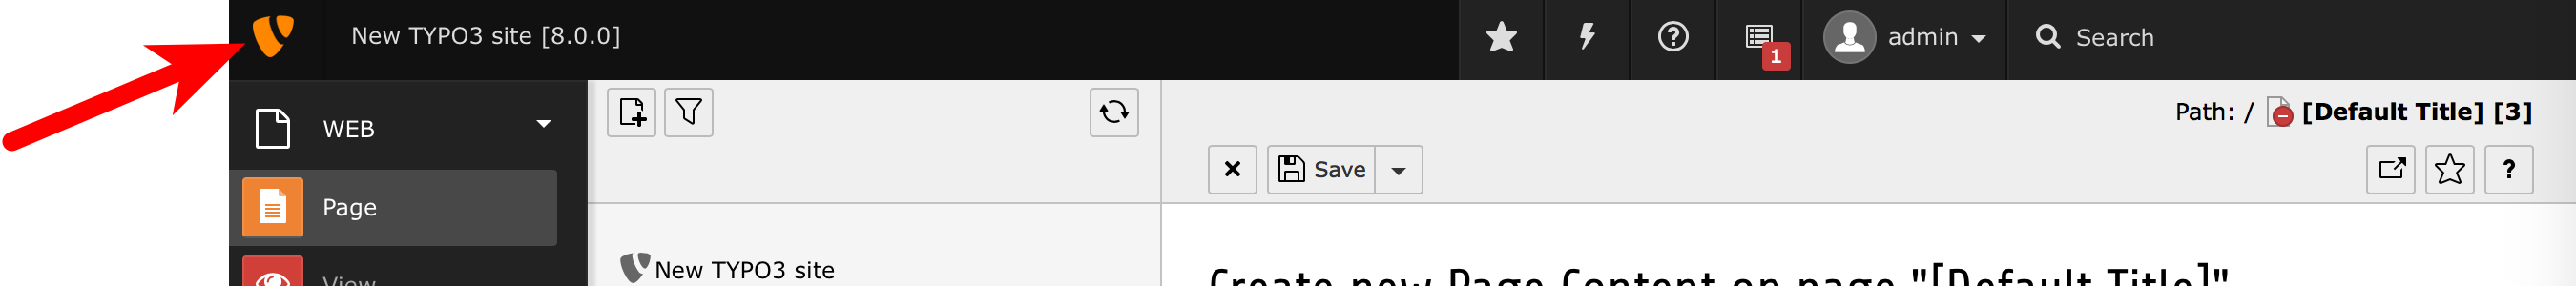
\includegraphics[width=0.7\linewidth]{BackendUserInterface/74109.png}
	\end{figure}

\end{frame}

% ------------------------------------------------------------------------------
% LTXE-SLIDE-START
% LTXE-SLIDE-UID:		ab5ef36b-c670fbea-fd6d762a-cb6f9195
% LTXE-SLIDE-TITLE:		Page module: drag and drop supports copying now
% LTXE-SLIDE-REFERENCE:	!Feature-74179-PageModuleDragDropCanDoCopiesViaCTRLKeyNow.rst
% ------------------------------------------------------------------------------
\begin{frame}[fragile]
	\frametitle{Backend User Interface}
	\framesubtitle{Kopieren von Seiten per Drag \& Drop}

	Zusätzlich zum Drag \& Drop Feature im Seitenmodul (womit man Inhaltselemente \textit{verschieben} konnte), ist es nun möglich diese auch zu kopieren, indem man zusätzlich die CTRL-Taste drückt. Nach der Operation lädt das Seitenmodul neu, damit alle Informationen aktualisiert werden.

	\begin{figure}
		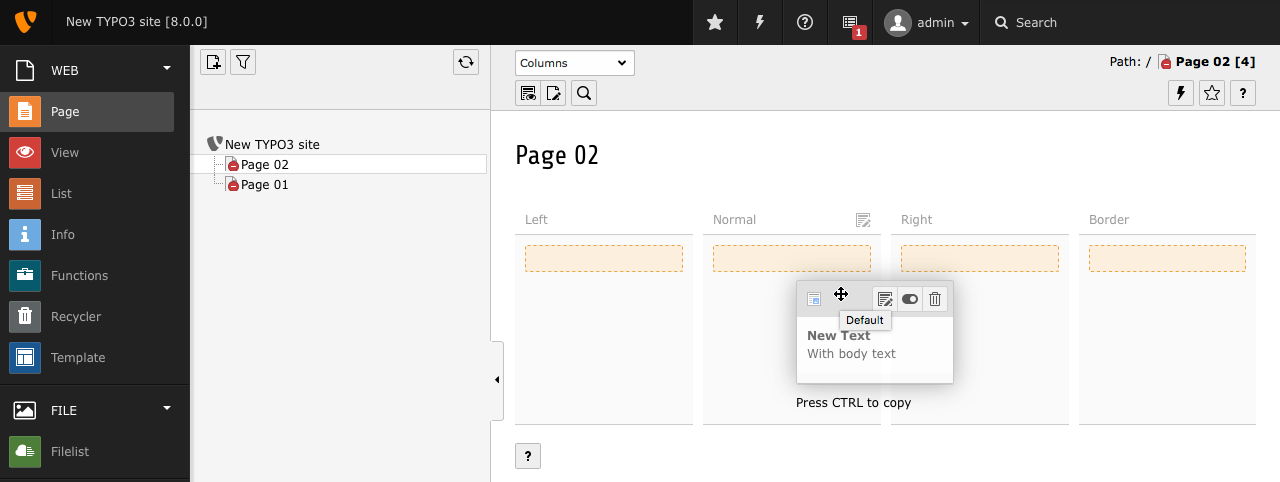
\includegraphics[width=0.7\linewidth]{BackendUserInterface/74179.png}
	\end{figure}

\end{frame}

% ------------------------------------------------------------------------------
